\documentclass[12pt]{extarticle}

\usepackage{fancyhdr,amsfonts,graphicx,wrapfig,sidecap,float,adjustbox,subcaption,indentfirst,amsmath,hyperref}
\usepackage{listings}
\usepackage{color}
\usepackage{gensymb}

\usepackage[right=2.5cm,left=2.5cm,top=2.5cm,bottom=2.5cm]{geometry}

\pagestyle{fancy}
\lhead{Memorial University of Newfoundland}
\rhead{Department of Mathematics and Statistics}
\renewcommand{\headrulewidth}{0.4pt}

\lfoot{Mathematics 2130}
\cfoot{}
\rfoot{Fall 2015, Project 2}
\renewcommand{\footrulewidth}{0.4pt}

\begin{document}
\begin{titlepage}
\vspace*{2in}
\begin{center}
{\LARGE The Oerth Project}
\end{center}

\vspace{2cm}

\abstract{This paper explores the dynamics of planetary projectile motion on Oerth, a fictional planet. Using Newton's laws and equations, projectile motion will be calculated. Including how trajectories change as velocities approach the escape velocity. It will discuss the deviation of expected and the actual distances over theta. Lastly, launching a projectile into orbit from surface is discussed. }


\vspace{3in}
\begin{flushright}
\begin{tabular}{l}
Project 2 \\
Mathematics 2130\\
Submitted by: John Hollett\\
Submitted to: Ivan Booth\\
\today
\end{tabular}
\end{flushright}


\end{titlepage}


\lhead{The Oerth Project}
\rhead{Math 2130}
\lfoot{John Hollett}
\rfoot{\thepage}
%\underheadoverfoot




\section{Introduction}
This paper observes a fictional planet called Oerth. Oerth is a planet with similar gravity, mass, and radius. Scientists want to build a weapon that can be used to fire at particular locations on the planet on any given day. This report will discuss these mechanics. This will be completed with a numerical analysis approach. 

Calculations are performed in the programming language C$^{\#}$. Graphing analysis is done using Maple plots. With C$^{\#}$, a utility was created for graphing the planetary projectile. It was used to find position of the projectile during each calculation. How this data was gathered and used is explained along with the physics used. 
 

\section{Equations}
This section explains the main details used to analyze trajectories of the projectile. The gravitational constant ($G$) and Oerth's mass ($M$) are consistently used in the calculations. Formulae for distance traveled ($R$) and force exerted by Oerth ($F$). Radius of Oerth ($r$) and the mass ($m$) of the object being fired. But, the mass of the projectile is neglected. This is due to the mass of the projectile being much smaller than Oerth.
\begin{align}
\label{R}
R &= \frac{v_o^{2}\sin{2\theta}}{g}, \text{Where } g = 10.0\text{ } m \cdot s^{-2}, v_o =  \text{ Initial Velocity} \\
\label{F}
F &= \frac{GMm}{r^{2}}, \text{Where } G = 6.67 \times 10^{-11}N\cdot m^{2}\cdot kg^{-2} \text{, \ \  } M = 5.40 \times 10^{24}kg \\
\label{Esc}
V_{Escape} &= \sqrt{\frac{2GM}{r}} \text{, and } V_{Orbital} = \sqrt{\frac{GM}{r}}
\end{align}



With projectile motion problems, there are two vector components in these equations. An $X$ and $Y$ component which make up a vector $\hat{U}$ which describes the positional vector. There is also a velocity vector $\hat{V}$ which is affected by the acceleration caused by gravity. Neglecting wind resistance, velocity parallel to the surface is not affected by gravity and is not reflected in these equations. Velocity also has an $X$ and $Y$ component. The escape velocity dictates the maximum magnitude possible at any angle from the center of the mass to the object's initial position. Any velocity greater than the escape velocity will be outside of Oerth's influence. There is also orbital velocity, which is the minimum required of any orbit at a particular radius from a mass.
\begin{align}
\label{U}
\hat{U} &= \hat{x} + \hat{y}\\
\label{V}
\hat{V} &= \hat{v_x} + \hat{v_y}
\end{align}

Where $t$ is time in relation to the current location of $\hat{x}$ and $\hat{y}$. For $\hat{v_x}$ and $\hat{v_y}$, it is velocity in relation to time. Lastly, $\varDelta{t}$ is the step change in time. Depending value used for $\varDelta t$, the accuracy of the projectile goes up or down in the numerical analysis of the projectile. The equations for finding each component of Equation (\ref{U}) and (\ref{V}) are as follows.
\begin{align}
\notag
\hat{x} = \hat{x}(t) + \hat{v_x}(t)\varDelta{t}\\
\notag
\hat{y} = \hat{y}(t) + \hat{v_y}(t)\varDelta{t}\\
\notag
\hat{v_x} = \hat{v_x}(t) + \ddot{x}\varDelta{t}\\
\notag
\hat{v_y} = \hat{v_y}(t) +\ddot{y}\varDelta{t}
\end{align}

The acceleration that affects these equations is part of Kepler's Law\cite{RVD}, Although, these listed here are simplified, they are based on a radial unit vector\cite{EMC} which is more complicated than what was used. A simplified version is used instead, which works for the purposes of this paper.

\begin{align}
\label{KXY}
\ddot{x} = -\frac{GM\hat{x}(t)}{(\hat{x}(t)^2+\hat{y}(t)^2)^{3/2}}\text{ and } \ddot{y} = -\frac{GM\hat{y}(t)}{(\hat{x}(t)^2+\hat{y}(t)^2)^{3/2}}
\end{align}

In the above, $\hat{x}(t)$ and $\hat{y}(t)$ are components of the positional vector $\hat{U}$ in Equation (\ref{U}) and where $t$ describes the current position at that point in time. These two acceleration functions are used to find the change in velocity vector $\hat{V}$ components in equation (\ref{V}). These values are then used to find the positional vector components in equation (\ref{U}).

\section{Analysis}

\subsection{Universal Constants and Expected Values}
Equation (\ref{R}) describes the expected distance based on angle and velocity. This can be tested numerically, and is within the scope of this report. The equation (\ref{F}) is used to find the force exerted on the projectile by Oerth. This force is derived by Equation (\ref{KXY}), which manipulates the acceleration of the particle launched given the current positional vector quantity from the center of Oerth.

The calculations dictate that for any velocity at which the projectile is launched, it must never exceed the escape velocity described by equation (\ref{Esc}). Should this occur, it would be lost into space. This is unlikely to happen due to the atmospheric penetration factor that would have to be at the correct angle, velocity and resistance to make it into space.\cite{NASA}


There are numerous equations that can be used to numerically solve projectile motion, but this report utilizes simplified versions. The equations used are sufficient to find data that can be utilized to prove the concepts in this paper.

\subsection{Launching Speeds}
In the Figure (\ref{fig:img1}) the projectile is traveling a short distance around Oerth. This is the first element of data collected. The initial velocity was approximately $200m\cdot s^{-1}$. Using Equation (\ref{R}), the result was $3,686.4m$. The actual numerical value is $3,678.472m$ which is less than the expected result. Figure (\ref{fig:img2}) had an initial velocity of $1000m\cdot s^{-1}$ and the result of equation (\ref{R}) was $100,000m$. The actual was $100,692.908m$. As the velocity of launch is increased, the values of $R$ become less accurate.
\begin{figure}[h!]
	\caption{Launching at Smaller Velocities}
	\begin{subfigure}{0.50\textwidth}
		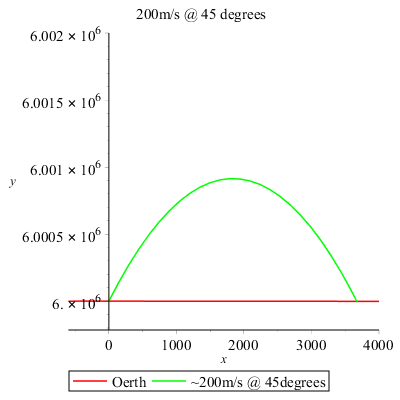
\includegraphics[scale=0.55]{First.png}
		\caption{$192m\cdot s^{-1}$ @ 45}
		\label{fig:img1}
	\end{subfigure}
	\begin{subfigure}{0.50\textwidth}
		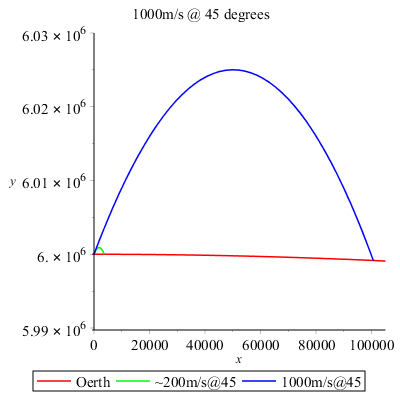
\includegraphics[scale=0.55]{Second.png}
		\caption{$1000m\cdot s^{-1}$ @ 45}
		\label{fig:img2}
	\end{subfigure}
\end{figure}
\begin{figure}[h!]
	\caption{Launching at Larger Velocities}
	\begin{subfigure}{0.50\textwidth}
		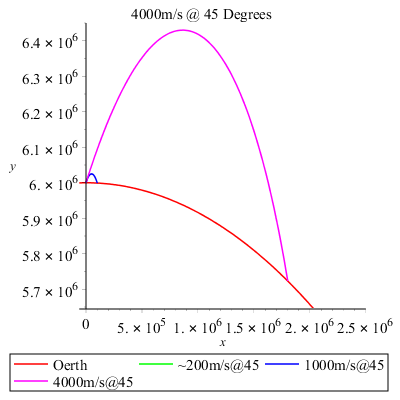
\includegraphics[scale=0.55]{Third.png}
		\caption{$4000m\cdot s^{-1}$ @ 45}
		\label{fig:img3}
	\end{subfigure}
	\begin{subfigure}{0.50\textwidth}
		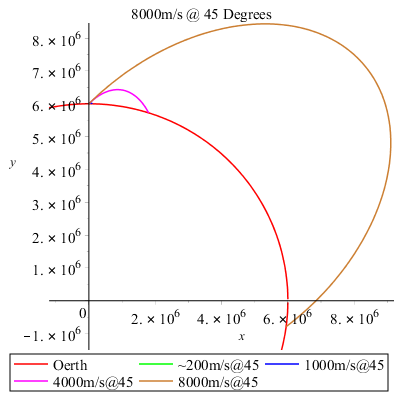
\includegraphics[scale=0.55]{Fourth.png}
		\caption{$8000m\cdot s^{-1}$ @ 45}
		\label{fig:img4}
	\end{subfigure}
\end{figure}

With the larger velocities in Figure (\ref{fig:img3}) and (\ref{fig:img4}), there are some early trends to observe regarding how the projectile is being launched.The first is the shifting of the $\hat{x}$ and $\hat{y}$ component acceleration on the particle. It does not become fully visible until larger $V_o$ values. It is important to note that these projectiles are different from those described in 2D-Kinematics because in this case gravity shifts from the $Y$-axis to the $X$-axis.


As the orbits get larger, more distance is traveled. Larger orbits take more time to complete a revolution if it does not escape Oerth's influence. When approaching the escape velocity, it takes more time to return as it becomes infinitesimally closer to this value. It is more difficult to calculate as it gets approaches escape velocity. This can be observed in figure (\ref{fig:img7}), where as the velocities get closer to $V_{Escape}$, they become more skewed elliptical in shape.

In figure (\ref{fig:img3}) and (\ref{fig:img4}), the larger values of initial velocity start to approach the speeds necessary to complete orbits or travel distances much further. To achieve half the distance around the planet, the projectile would need to be launched closer to the surface. To launch a projectile around the earth, the gravity needs to be utilized to manage longer distances. This can also be seen in the figure (\ref{fig:img4}). The angle is just as important as the velocity. The advantage of launching projectiles at angles closer to the surface makes use of gravity to slingshot it around the planet much easier. 

\subsection{R vs Theta}
\begin{figure}[h!]
	\caption{R vs Theta}
	\begin{subfigure}{0.50\textwidth}
		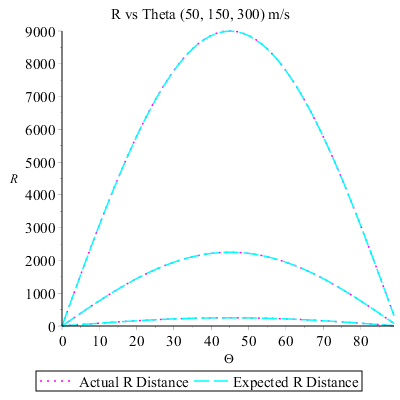
\includegraphics[width=0.8\linewidth]{RvsTheta1.png}
		\caption{Smaller Velocities}
		\label{fig:img5}
	\end{subfigure}
	\begin{subfigure}{0.50\textwidth}
		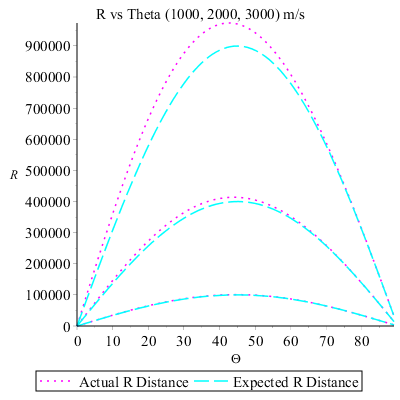
\includegraphics[width=0.8\linewidth]{RvsTheta2.png}
		\caption{Larger Velocities}
		\label{fig:img6}
	\end{subfigure}
	
\end{figure}
In Figure (\ref{fig:img5}), there is a relationship between R, which is the distance traveled along the surface, and Theta, which is the angle of launch. This figure contains the launch velocities $50$$m \cdot s^{-1}$, $150$$m \cdot s^{-1}$ and $300$$m \cdot s^{-1}$. To make it easier to see the relation between these velocities, two colors and different style lines were used. This is important because at lower velocities, this relationship stays true. Using the equation (\ref{R}), the data stays within an acceptable error at these velocities. It is not exact, but it is adequately close.

When examining figure (\ref{fig:img6}) there is a noticeable change. It represents the speeds $1000$$m \cdot s^{-1}$, $2000$$m \cdot s^{-1}$ and $3000$$m \cdot s^{-1}$. After $2000$$m \cdot s^{-1}$ the actual $R$ distance changes substantially. And as this change is noticeable early in velocities leading up to $V_{Escape}$, it is expected this deviation will be larger as it approaches $V_{Escape}$. Differences in these values is more noticeable at the 45$^{\circ}$ angle. There is also bias towards velocities at angles $0^{\circ} \leq \varTheta < 45^{\circ}$.

It is important to make this distinction between actual and expected $R$ values. The shifting gravity and decline in the surface affects the projectile's $R$ distance as velocities increase. To quantify this from equation (\ref{R}), as $v_{o} \to (V_{Orbital} \lor V_{Escape})$ with $0^{\circ} \leq \varTheta < 45^{\circ}$, it will deviate increasingly.


\subsection{Orbital Plausibility}
This section describes whether or not it is possible to put a projectile into an orbit from the surface. The short answer is yes. However, this does not come without complications. The approach to this problem also matters significantly. 

To calculate this numerically, $\varDelta t$ needs to be low so that it is accurate enough to eliminate some of the error that occurs doing this in steps. To ensure that the calculations are successful, the initial height must be increased. However, this means the projectile is no longer launched from the surface. The safest value found was at least five meters above the surface. A circular orbit is possible with no ellipse, however it is required to be launched at zero degrees to the surface. The velocity needs to be sufficient to negate the gravity of Oerth. This was found to be approximately $7748 m\cdot s^{-1}$.

\begin{wrapfigure}[21]{r}{0.485\textwidth}
	\begin{center}
		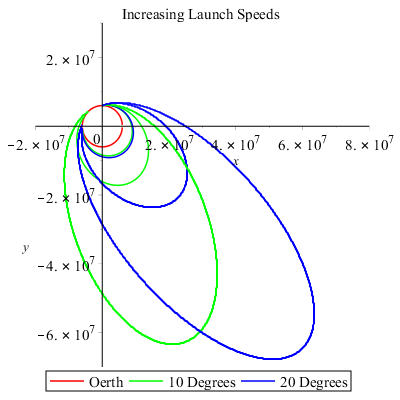
\includegraphics[scale=0.55]{Vescape.png}
		\caption{Increasing velocities @ 10 and 20 degrees}
		\label{fig:img7}
	\end{center}
\end{wrapfigure}

Using more rigorous testing, the results are proof that it is possible. While this is certainly possible, the test assumes the surface is perfectly spherical. The path of the projectile would need to be free of obstacles in its path. This test neglects wind resistance as well. This would be impossible in real scenarios.

In an elliptical orbit, some of these concerns are alleviated. However, if the orbit is large enough to hit the atmosphere it will burn the projectile. 

Achieving an orbit from the surface is impossible. Launching at the surface, the projectile will return to the position it originated from which would be the surface itself. This is shown in figure (\ref{fig:img7}). These trends will not change at orbital velocity. Ignoring these problems entirely and launching the projectile above the surface makes an orbit possible. 

Assuming that the cannon is above the ground or raised up and lowered after a launch makes this possible. In a perfect circular orbit initiated at the surface, the orbit itself would the surface. In an elliptic orbit, it still makes contact with the surface after a completed orbit. It is improbable to get a proper orbit from the surface under real conditions. However, it can also be said it is not impossible either under the right conditions.

\section{Technical Details}

This section describes the calculations that have been used. Using the code referenced in the index created from the sources listed and project details, the data was calculated. This allowed data to be plotted as accurately as possible given a $\varDelta t$.

The calculations that take place are carried out within a defined object. This object has its own values for the relevant launch. It has properties defined like magnitude, $V_{Orbit}$ and $V_{Escape}$ to help accuracy. It takes $\hat{x}$ and $\hat{y}$ from equation (\ref{U}) as part of the initial position. A velocity and angle is given in order to calculate $\hat{v}_x$ and $\hat{v}_y$ for equation (\ref{V}). This is done using the commonly used Pythagoras theorem.

These calculations come with serious drawbacks. One of the most profound observations is the lack of accuracy in higher valued changes in time. This affects calculations done with change in time stepping greater than half a second. This produces less accurate results. Even lower values than this can still be enough to throw off the accuracy depending on velocity. The reason for this is at the position where each point is recorded, the next point acts like a line with length determined by the value of $\varDelta t$. 

This can cause the calculations at each step to change the $X$ and $Y$ components of the $\hat{U}$ vector. During the period between calculations, changes that should be happening with the gravity do not happen until the next step in calculation. To visualize this, it is similar to using a series of lines to create a circle. It will not be rounded. Using increasingly shorter lines makes for a rounder circle.

During each calculation, a step function is used which is defined to calculate velocity and acceleration before applying it to the position. This happens at each change in time defined by $\varDelta t$. Using some rough scaling, the number of points is reduced but, the accuracy of the calculations is unchanged.
To calculate the radians around Oerth, the well known equation was used:
\begin{equation}
\notag
cos\ \varTheta = \frac{\hat{F} \cdot \hat{G}}{\|\hat{F}\|\ \|\hat{G}\|}
\end{equation}

With this equation, using conditional statements, the distance around the surface of Oerth is found. This works for the numerical analysis of $R$ in equation (\ref{R}) because, $R$ does not take into account the circular properties of Oerth or other scenarios.

\section{Conclusion}

The dynamics of projectile motion on a planetary scale, while very similar, has differences. Some of these are the limits of the velocity and angles these projectiles can have. The escape velocity plays a part in determining a speed limit, relative to the distance from planets. Simple physics formulae used in basic kinematics are sufficient for the low-scale, but on the larger-scale, more advanced methods are necessary. Without these it would not be possible to accomplish much space exploration and much more.

The projectile motion that is used in this report does not fully convey how important these calculations are. The laws these formulae are derived from are used in calculations involving satellite motion and whether or not orbits are clear of any intersecting objects, like space stations and so on. 

If these methods for calculating motion did not exist, devastating accidents could occur more frequently. Objects moving at the speed necessary to maintain orbit, makes for deadly collisions that can easily destroy objects such as space stations. Debris that this creates is mutually assured to be destructive to anything else in its path.

Furthermore, when these laws and formulae are used to their full potential, they can calculate and plan long distance space travel. The probes sent to space use orbital dynamics and escape velocities to project paths to other masses in space like a slingshot.

Understanding of these concepts is important for the future of space travel and exploration. They will always play a role in models of space exploration. Many of these mechanics are quantified to explain behaviors of the visible universe. These equations as a result, must be appreciated.
\newpage

\lstset{basicstyle=\footnotesize,breaklines=true}
\lstset{framextopmargin=50pt,frame=bottomline}

\section{C$^{\#}$ Code}
\lstinputlisting[caption=KeplerProjectile.cs]{Kepler.cs}
\newpage
\begin{thebibliography}{99}

\bibitem{wiki}"Newton's Laws of Motion" Wikipedia: The Free Encyclopedia. Wikimedia Foundation, Inc. 13 Oct 2015. Web. 18 Oct 2015
\bibitem{NASA}"Atmospheric Flight" NASA History. \url{http://history.nasa.gov/conghand/atmosphe.htm} National Aeronautics and Space Administration, Web. 20 Oct 2015
\bibitem{EMC}"Elementary Mathematical and Computer Tools for Electrical and Computer Engineers Using MATLAB" Jamal T. Manassah. \url{https://books.google.ca/books?id=qGEImarSDDIC&pg=PA260#v=onepage&q&f=false} Taylor \& Francis Group, 2007, Web. 21 Oct 2015
\bibitem{RVD}"The Radial Velocity Equation" Department of Physics \& Astronomy \url{http://w.astro.berkeley.edu/~kclubb/pdf/RV_Derivation.pdf} San Francisco State University, Aug 2008, Web. 21 Oct 2015

\end{thebibliography}

\end{document}
